\documentclass[12pt]{article}
\usepackage[a4paper,margin=2.5cm]{geometry}
\usepackage{fontspec}
\IfFontExistsTF{Arial}{\setmainfont{Arial}}{\setmainfont{TeX Gyre Heros}}
\usepackage{graphicx,booktabs,array,tabularx,url,microtype,amsmath}
\usepackage[colorlinks=true,allcolors=blue]{hyperref}
\setlength{\emergencystretch}{2em}
\renewcommand{\baselinestretch}{1.2}
\title{Supplementary Information\\Donor-aware cross-cohort transcriptomics prioritizes P2RX4 in human diabetic retinopathy}
\author{Mengjiao Wang, Xiaoyan Zhao, Xincheng Sun, Pingan Mao}
\date{}

\begin{document}
\maketitle
\renewcommand{\thefigure}{S\arabic{figure}}

\section{Supplementary-table map}

The consolidated workbook contains only results used by this Research Article. Tables are numbered S1--S28 and are reproducible from the included final scripts.

\begin{tabularx}{\dimexpr\textwidth-18pt\relax}{@{}p{0.12\textwidth}X@{}}
\toprule
Item & Description\\
\midrule
S1 & Donor-aggregated GSE160306 metadata and expression for 158 inflammatory genes\\
S2 & Total-association and DME-conditioned HC3+$t$ models with wild-bootstrap-$t$ results\\
S3 & Primary total-association ranking, candidate tiers, resampling, and influence summaries\\
S4 & Two thousand stage-stratified donor-bootstrap coefficient and rank summaries\\
S5 & Leave-one-donor coefficient and rank summaries for all 158 genes\\
S6 & Candidate-level leave-one-donor detail\\
S7 & Candidate leverage, Cook's distance, and severity DFBETA\\
S8 & Design leverage for all 26 donors\\
S9 & Worst-eye, rank, stage, high-leverage exclusion, DME-conditioned, and Huber sensitivities\\
S10 & Exploratory P2RX4 severity-by-DME interaction\\
S11 & Five clinical contrasts with within-family and global multiplicity correction\\
S12 & GSE102485 membrane-only post-hoc context\\
S13 & GSE102485 deposited sample annotations\\
S14--S15 & Nested donor-level prediction rows and summary metrics\\
S16 & Retrospectively reconstructed external-dataset search, eligibility, and scope log\\
S17 & Patient/sample-level P2RX4 values for three separate GEO datasets\\
S18 & External P2RX4 effects, tests, intervals, and adjusted sensitivities\\
S19 & Independent-validation leave-one-patient/sample-out direction analyses\\
S20 & Frozen-protocol deviations and consequences\\
S21 & Voigt et al. author-cluster mapping\\
S22 & Normal-retina library dominance and donor-aggregated candidate localization\\
S23 & Normal-retina leave-one-donor dominance\\
S24 & Normal-retina between-donor descriptive ranges\\
S25 & GSE276892 reconstructed-count P2RX4 negative-binomial models\\
S26 & GSE276892 reconstructed sample counts, QC correlations, reference sensitivity, and integrity\\
S27 & GSE179568 clinical-covariate sensitivity models\\
S28 & GSE179568 covariate balance and public-metadata patient-overlap audit\\
\bottomrule
\end{tabularx}

\section{Discovery-model details}

\subsection{Two estimands}

The total-association model omits DME and asks how expression varies with donor-level retinal severity after demographic and tissue-quality adjustment. The DME-conditioned model adds DME and asks how expression varies with severity among donors with the same observed DME status. In cross-sectional data, DME can plausibly be a correlate, mediator, or consequence; therefore the second model is not described as uniquely deconfounded. The two complete 158-gene result sets are presented side by side in S2.

\subsection{Finite-sample inference}

All HC3 model tests use the Student $t$ distribution with residual degrees of freedom (20 for the primary total-association model and 19 for the DME-conditioned model). Wild-bootstrap-$t$ resampling used 4,999 Rademacher multipliers applied to HC3-scaled residuals from the null model. Two-sided empirical $P$ values were calculated as $(1+\sum I(|t^*|\ge |t|))/(B+1)$. This sensitivity addresses heteroskedasticity more directly than exchangeable residual permutation. Benjamini--Hochberg adjustment covered 158 genes per severity estimand.

\subsection{Severity aggregation and alternative encodings}

The source values 10, 20, 35, 43, 53, and 65 are ordered ETDRS DR severity levels. Three paired-eye donors occurred in the diabetes-only discovery cohort. Two had identical eye-specific scores; the third had 35 and 43, giving a donor mean of 39. The primary mean rule matches donor-mean expression but assumes an approximately linear relationship across numeric levels. S9 therefore includes worst-eye severity, midrank severity, and a clinical-stage code (diabetes without DR=0, NPDR=1, PDR=2). P2RX4 ranked first under mean, worst-eye, and rank representations and second under stage coding.

\subsection{Influence and candidate tiers}

Leverage depends only on the primary design matrix. Donor \texttt{13\_030} exceeded $2p/n$ with leverage 0.771 and PMI 149 minutes. S7 and S8 provide leverage, Cook's distance, and severity DFBETA. Removing this donor left P2RX4 at rank 1. Candidate tiers were assigned after examining the two estimands and resampling: P2RX4 is discovery-selected and evaluated as the sole external target; CD82, NLRP3, and FPR1 are cross-estimand secondary candidates; TLR2 and SLC31A1 are estimand-dependent; all other genes are unprioritized. These tiers are descriptive and are not significance thresholds.

\section{Multiplicity and predictive falsification}

The NPDR-without-DME versus diabetes-without-DR contrast is the primary 158-gene contrast family because neither group has DME. The other four contrasts are exploratory. S11 gives both within-contrast FDR and a global 790-test FDR sensitivity. Covariate-adjusted PDR estimates are not calculated with two case donors.

The classification target, any DR versus diabetes without DR, differs from the continuous severity estimand. It is therefore restricted to S14--S15 as a falsification audit. Ranking, residualization, scaling, and model fitting occur inside each training fold. AUC is accompanied by Brier score and log loss and is not reported in the abstract.

\section{Independent-validation protocol and deviations}

P2RX4 was the sole target in a locally retained protocol. The authors state that it was specified before processed GSE276892 values were inspected. Its SHA-256 is {\footnotesize\texttt{FA0EBEEF\allowbreak E4570917\allowbreak 8E197B6F\allowbreak 0819F7AA\allowbreak 1E1692E5\allowbreak 0AA2C7F4\allowbreak 7E2601D7\allowbreak CA3C8EED}}. The hash authenticates present content but supplies no independent creation timestamp; this is not public preregistration. The protocol specified a negative-binomial count model with a one-sided Wald test but did not specify FASTQ alignment, annotation, lane aggregation, or quantification. The deposited matrix contains DESeq2-normalized values, so refitting a count model to it would be invalid. Instead, available raw reads were reconstructed as a post-protocol preprocessing deviation.

The reconstruction aligned 10 GSE276892 runs and 21 GSE147657 lanes with STAR 2.7.8a and counted genes with featureCounts 2.0.1. The source-faithful workflow used GENCODE release 42 GRCh38.p13 all-regions FASTA and annotation; a primary-assembly workflow served as a reference sensitivity. Technical lanes were summed to the 17 deposited biological profiles. The archive SHA-256 was {\footnotesize\texttt{CF6784D6\allowbreak 852D30A7\allowbreak A2A67FDF\allowbreak C0C7FB93\allowbreak E0A3ABBF\allowbreak 3207CE77\allowbreak 5F860709\allowbreak 795D65A6}}; all 442 internal workflow hashes passed.

The all-regions disease-only negative-binomial estimate for P2RX4 was log$_2$ fold change 0.295 (95\% CI $-0.854$ to 1.443; two-sided Wald $P=0.615$; one-sided $P=0.308$); the primary-assembly estimate was 0.289 ($P=0.622$). Age/sex, reused-source, source+age/sex, PDR\_S10 exclusion, and 8-versus-2 new-profile sensitivities all retained positive point estimates but wide intervals. PDR\_S10 had six P2RX4 reads, compared with 2,074--7,153 among the other PDR profiles. Removing it increased the estimate to 0.496 but remained non-significant (two-sided $P=0.105$). Reference-pair P2RX4 counts differed by at most one read per sample. Raw P2RX4 counts were strongly associated with assignment, total gene counts, mapping rate, and size factor, as expected for unnormalized counts. Size-factor-normalized P2RX4 retained an inverse association with detected genes ($\rho=-0.591$, BH-adjusted $P=0.0451$ across 18 QC/clinical correlations). These results make GSE276892 evaluable but inconclusive; they do not turn the reconstruction into a preregistered confirmation.

GSE179568 and GSE94019 were identified and added after the local protocol. The reconstructed search log is retrospective, and contemporaneous records do not establish whether P2RX4 values were unseen before the post-protocol dataset decisions. All their inferential $P$ values are therefore two-sided and exploratory, with Holm adjustment across the three designated post-protocol primary comparisons. Public GSE276892/GSE179568 metadata show a shared Freiburg context, no exact sample-label overlap, and three exact PDR age/sex matches; anonymization, missing surgery identifiers, and absent author confirmation prevent proof or exclusion of patient overlap. The manuscript consequently uses ``separate GEO datasets,'' not ``independent patients.''

For GSE179568, clinical rows were transcribed from source Supplementary Table 1 and linked in deposited matrix order. PDR ages were 20--60 years, macular-pucker ages 62--83, and macular-hole ages 61--79; neither control comparison had age common support. The unadjusted RNV-versus-macular-pucker HC3 coefficient was 0.696 ($P=0.0315$), compared with 0.102 ($P=0.773$) after age/sex adjustment, 0.202 ($P=0.570$) using age/sex Huber regression, and 0.464 ($P=0.114$) after adding prior PRP, anti-VEGF, and vitrectomy. These regressions extrapolate outside observed age support and cannot resolve disease from age, treatment, or cell composition. Propensity weighting was not attempted because positivity was absent.

\begin{figure}[h!]
\centering
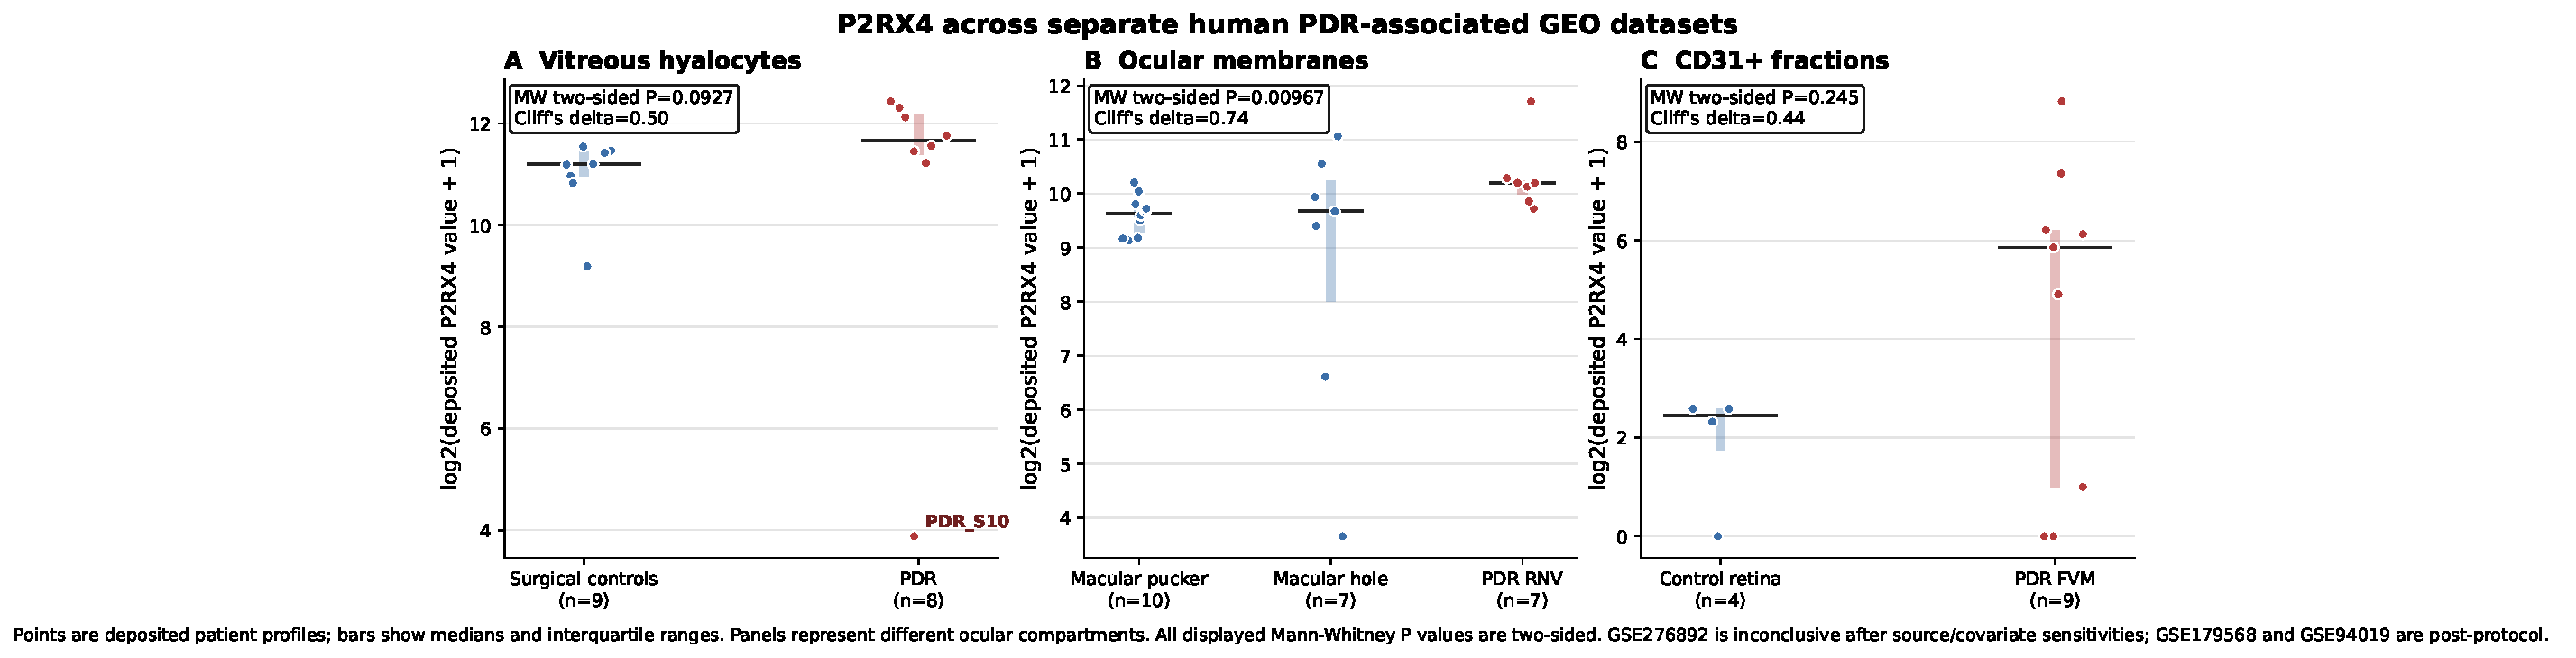
\includegraphics[width=\textwidth]{../figures/Figure_4_independent_P2RX4_validation.pdf}
\caption{Processed-value P2RX4 distributions in separate GEO datasets. Bars show patient-profile medians and interquartile ranges; all displayed Mann--Whitney $P$ values are two-sided. These panels do not show the reconstructed negative-binomial model or remove source, age, treatment, or tissue-composition confounding.}
\end{figure}

\begin{figure}[h!]
\centering
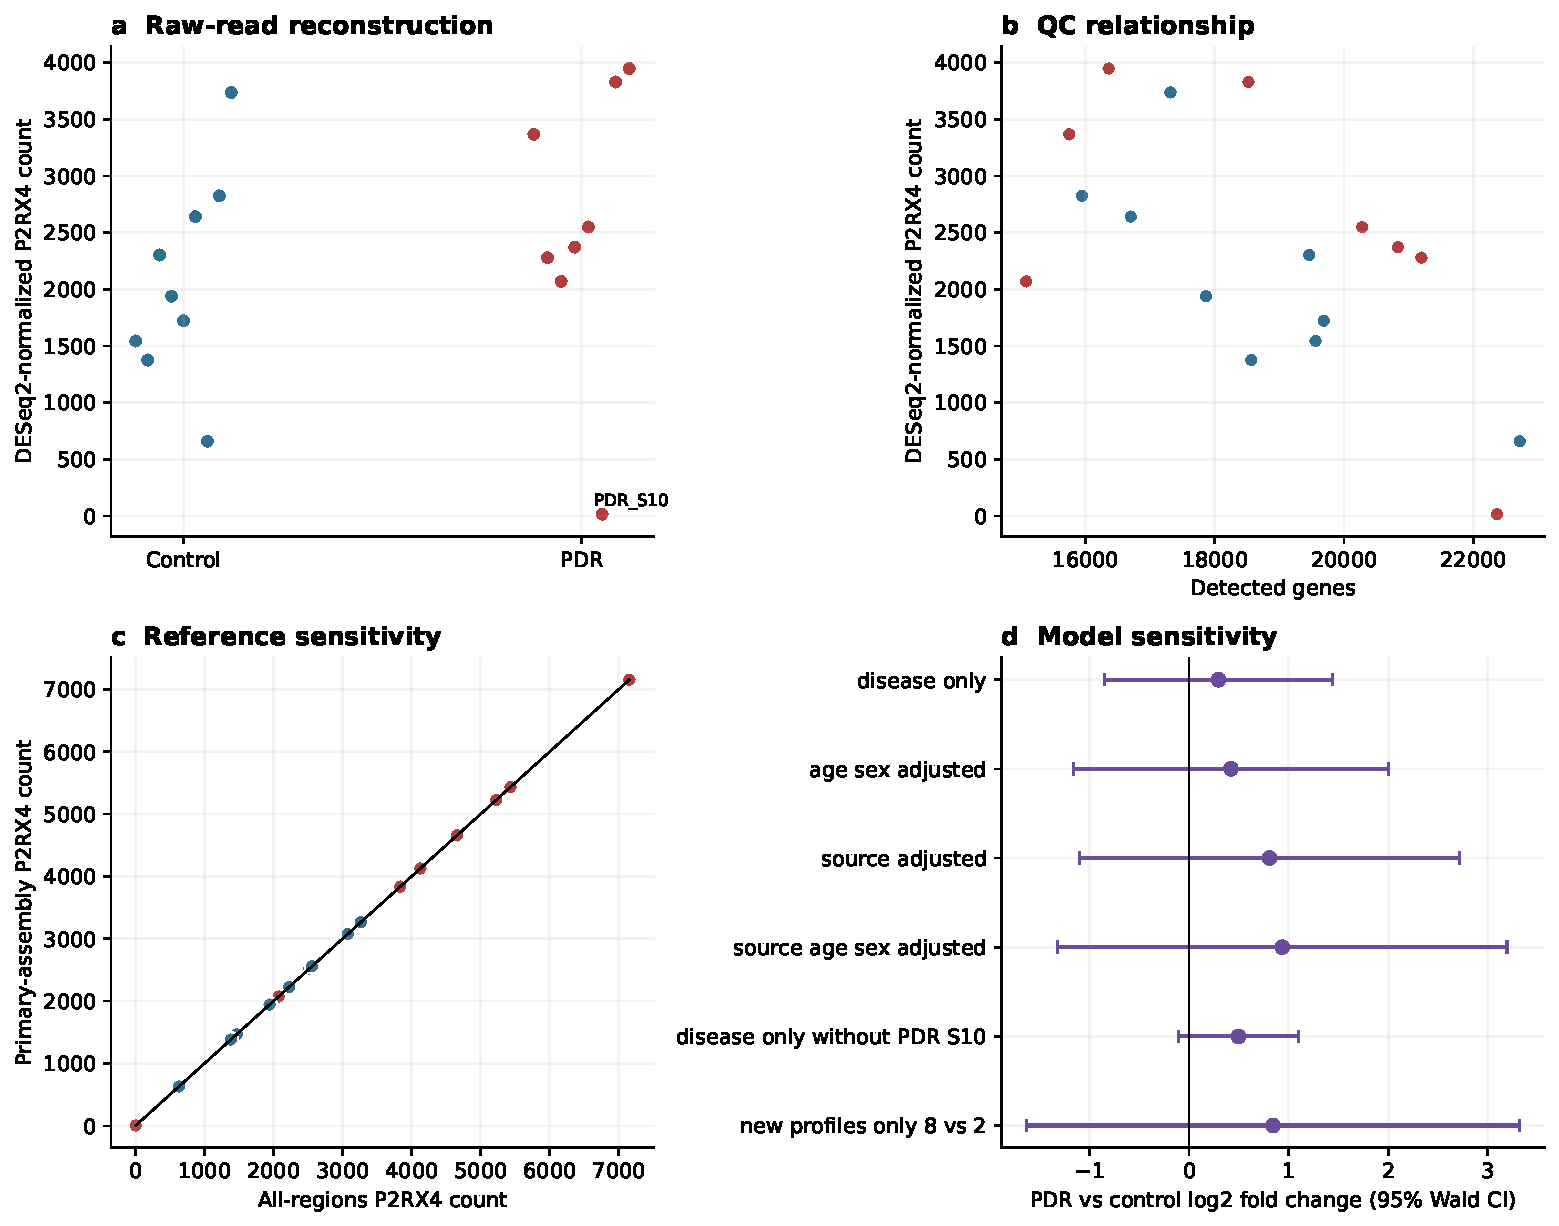
\includegraphics[width=\textwidth]{../figures/Supplementary_Figure_raw_count_reconstruction.pdf}
\caption{GSE276892 raw-read reconstruction. The figure reports reconstructed P2RX4 counts, negative-binomial effect estimates, source/reference sensitivities, and the exceptionally low PDR\_S10 profile. The workflow was specified after target selection and is a protocol deviation.}
\end{figure}

\begin{figure}[h!]
\centering
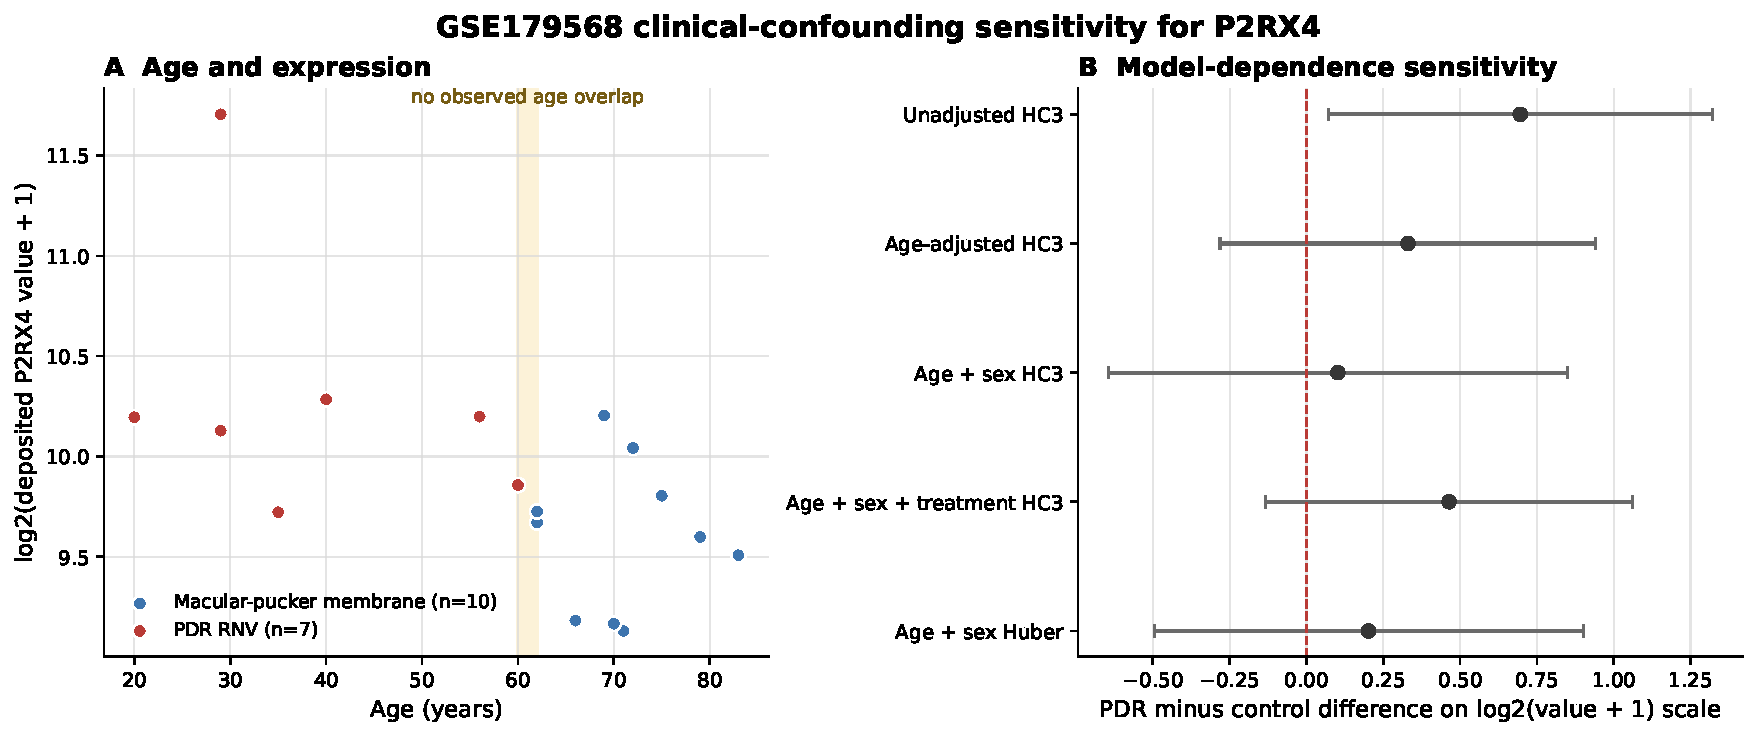
\includegraphics[width=\textwidth]{../figures/Supplementary_Figure_GSE179568_clinical_sensitivity.pdf}
\caption{GSE179568 clinical-confounding sensitivity. (a) P2RX4 expression by age shows no observed age overlap between PDR RNV and macular-pucker membrane groups. (b) Unadjusted, HC3-adjusted, and Huber coefficients are model dependent; adjusted estimates extrapolate beyond observed age support.}
\end{figure}

\section{Normal-retina localization boundary}

GSE130636 comprises six donor-region libraries from three normal donors. The descriptive atlas panel is the ordered six-gene union of both primary-estimand top-five sets: P2RX4, TLR2, CD82, NLRP3, FPR1, and SLC31A1. Atlas values were not fed back into ranking. Summaries were first calculated within library and author-mapped cell type, then averaged across fovea and periphery within donor. Leave-one-donor dominance recalculated the highest mean cell type after removing each donor. P2RX4 pooled dominance was microglial but agreed in one of three folds; the other folds were amacrine dominant. TLR2, NLRP3, and FPR1 were microglia-dominant in all three folds, CD82 was M\"uller-enriched-glia dominant in all folds, and SLC31A1 was endothelial-dominant in two. Between-donor intervals are minimum--maximum descriptive ranges, not population confidence intervals. No normal-retina result is treated as disease-state replication or disease-state cellular origin.

\begin{figure}[h!]
\centering
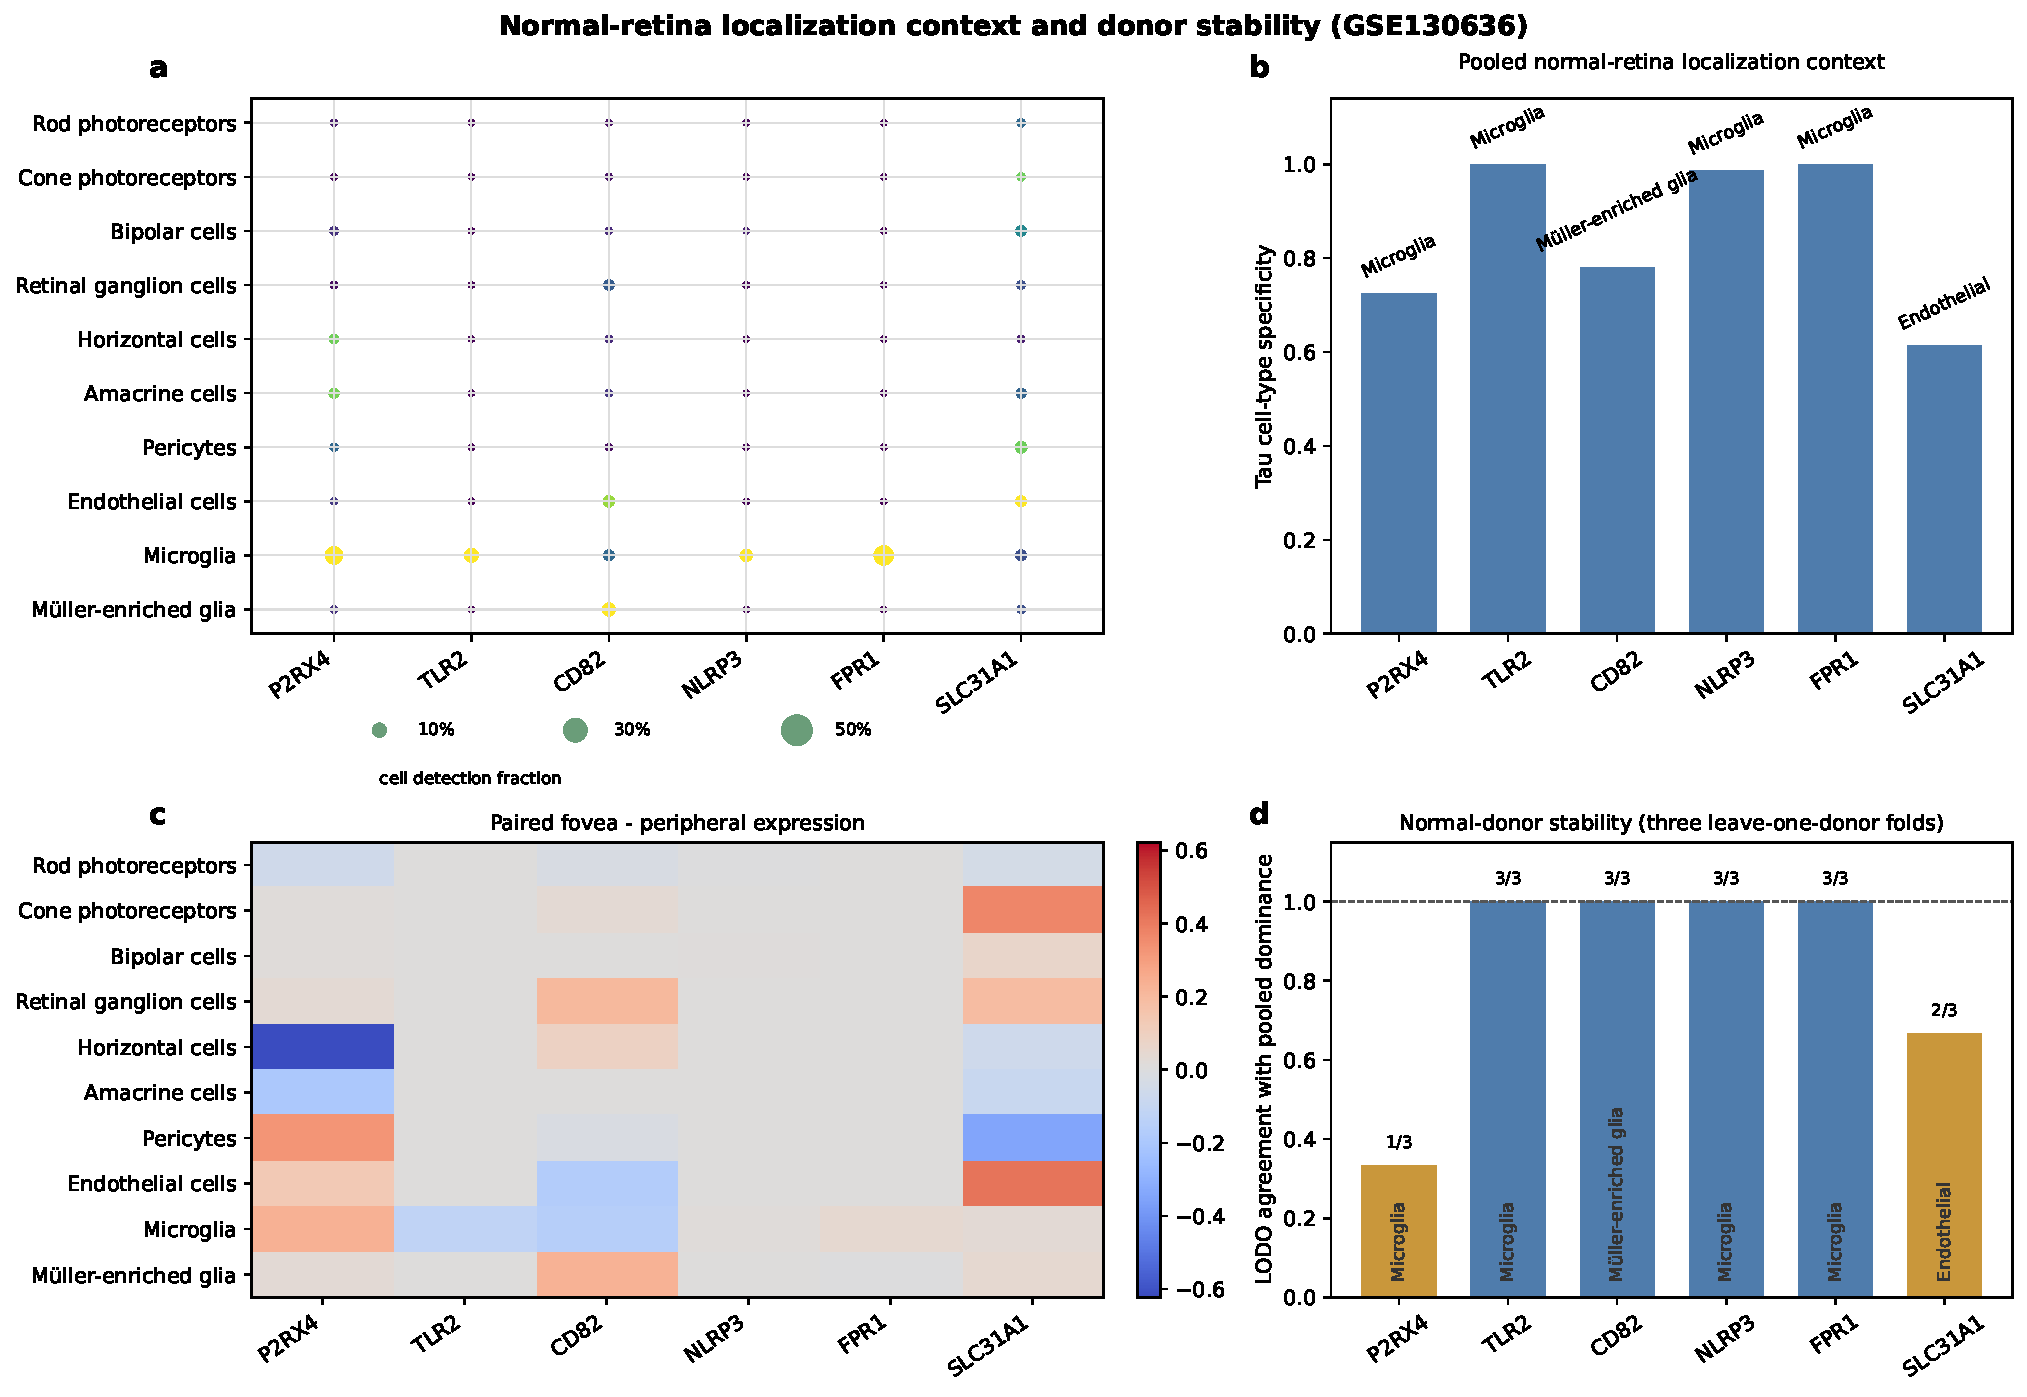
\includegraphics[width=\textwidth]{../figures/Figure_5_cell_type_localization.pdf}
\caption{Normal-retina localization context and donor stability. Expression, detection, regional differences, and leave-one-donor dominance are computed from author-mapped GSE130636 libraries.}
\end{figure}

\section{Anatomical and statistical claim boundaries}

The evidence levels are: (1) adjusted severity association in the GSE160306 inflammatory search space; (2) stability and influence within that same discovery cohort; (3) single-target observations in separate human PDR-associated ocular datasets, including an inconclusive post-protocol raw-read reconstruction and a clinically confounded membrane comparison; and (4) descriptive localization in normal retina. The analysis does not establish patient independence across Freiburg datasets, whole-retina replication, P2RX4 cellular exclusivity, intercellular communication, diagnostic performance, therapeutic efficacy, or causality.

\end{document}
